
%% bare_conf.tex
%% V1.3
%% 2007/01/11 
%% by Michael Shell
%% See:
%% http://www.michaelshell.org/
%% for current contact information.
%%
%% This is a skeleton file demonstrating the use of IEEEtran.cls
%% (requires IEEEtran.cls version 1.7 or later) with an IEEE conference paper.
%%
%% Support sites:
%% http://www.michaelshell.org/tex/ieeetran/
%% http://www.ctan.org/tex-archive/macros/latex/contrib/IEEEtran/
%% and
%% http://www.ieee.org/


\documentclass[10pt, conference]{IEEEtran}
% \usepackage{blindtext, graphicx}
\usepackage{graphicx}

% Add the compsoc option for Computer Society conferences.
%
% If IEEEtran.cls has not been installed into the LaTeX system files,
% manually specify the path to it like:
% \documentclass[conference]{../sty/IEEEtran}


% *** CITATION PACKAGES ***
%
\usepackage{cite}
% cite.sty was written by Donald Arseneau
% V1.6 and later of IEEEtran pre-defines the format of the cite.sty package
% \cite{} output to follow that of IEEE. Loading the cite package will
% result in citation numbers being automatically sorted and properly
% "compressed/ranged". e.g., [1], [9], [2], [7], [5], [6] without using
% cite.sty will become [1], [2], [5]--[7], [9] using cite.sty. cite.sty's
% \cite will automatically add leading space, if needed. Use cite.sty's
% noadjust option (cite.sty V3.8 and later) if you want to turn this off.
% cite.sty is already installed on most LaTeX systems. Be sure and use
% version 4.0 (2003-05-27) and later if using hyperref.sty. cite.sty does
% not currently provide for hyperlinked citations.
% The latest version can be obtained at:
% http://www.ctan.org/tex-archive/macros/latex/contrib/cite/
% The documentation is contained in the cite.sty file itself.


% *** GRAPHICS RELATED PACKAGES ***
%
\ifCLASSINFOpdf
  % \usepackage[pdftex]{graphicx}
  % declare the path(s) where your graphic files are
  % \graphicspath{{../pdf/}{../jpeg/}}
  % and their extensions so you won't have to specify these with
  % every instance of \includegraphics
  % \DeclareGraphicsExtensions{.pdf,.jpeg,.png}
\else
  % or other class option (dvipsone, dvipdf, if not using dvips). graphicx
  % will default to the driver specified in the system graphics.cfg if no
  % driver is specified.
  % \usepackage[dvips]{graphicx}
  % declare the path(s) where your graphic files are
  % \graphicspath{{../eps/}}
  % and their extensions so you won't have to specify these with
  % every instance of \includegraphics
  % \DeclareGraphicsExtensions{.eps}
\fi
% graphicx was written by David Carlisle and Sebastian Rahtz. It is
% required if you want graphics, photos, etc. graphicx.sty is already
% installed on most LaTeX systems. The latest version and documentation can
% be obtained at: 
% http://www.ctan.org/tex-archive/macros/latex/required/graphics/
% Another good source of documentation is "Using Imported Graphics in
% LaTeX2e" by Keith Reckdahl which can be found as epslatex.ps or
% epslatex.pdf at: http://www.ctan.org/tex-archive/info/
%
% latex, and pdflatex in dvi mode, support graphics in encapsulated
% postscript (.eps) format. pdflatex in pdf mode supports graphics
% in .pdf, .jpeg, .png and .mps (metapost) formats. Users should ensure
% that all non-photo figures use a vector format (.eps, .pdf, .mps) and
% not a bitmapped formats (.jpeg, .png). IEEE frowns on bitmapped formats
% which can result in "jaggedy"/blurry rendering of lines and letters as
% well as large increases in file sizes.
%
% You can find documentation about the pdfTeX application at:
% http://www.tug.org/applications/pdftex


% correct bad hyphenation here
\hyphenation{op-tical net-works semi-conduc-tor}
\IEEEoverridecommandlockouts
\usepackage{url}



\begin{document}
%
% paper title
% can use linebreaks \\ within to get better formatting as desired
\title{An API Honeypot for DDoS and XSS Analysis}


% author names and affiliations
% use a multiple column layout for up to three different
% affiliations
\author{\IEEEauthorblockN{G Leaden, Marcus Zimmermann, Casimer DeCusatis, \textit{Fellow, IEEE}, and Alan G. Labouseur}
\IEEEauthorblockA{School of Computer Science and Mathematics\\
Marist College\\
Poughkeepsie, NY 12601\\
\{G.Leaden1, Marcus.Zimmermann1, Casimer.DeCusatis, Alan.Labouseur\}@Marist.edu 
\thanks{This work was supported by the National Science Foundation under CC*DNI Integration (Area 4): Application Aware Software-Defined Networks for Secure Cloud Services (SecureCloud). Award \#1541384.}}
}


% make the title area
\maketitle


\begin{abstract}
Honeypots are systems built to mimic critical parts of a network, distracting attackers while logging their information to develop attack profiles. This paper discusses the design and implementation of a honeypot disguised as a REpresentational State Transfer (REST) Application Programming Interface (API). This honeypot was deployed as part of the NSF SecureCloud test bed.  We discuss the motivation for this work, design features of the honeypot, and experimental data showing performance under various traffic conditions.  We also present the analysis of both a distributed denial of service (DDoS) attack and a cross-site scripting (XSS) malware insertion against this honeypot.
\end{abstract}

%!TEX root=main.tex

\section{Introduction} \label{intro}

The number and severity of cyber attacks has grown significantly in recent years~\cite{Symantec-Threat-Report,IBM-XForce-Report}. 
Cyber attackers have managed to pull off virtual bank heists, distributed denial of service (DDoS) attacks powered by botnets and Internet of Things (IoT) devices, and power outages caused by malware~\cite{IBM-XForce-Report}. 
Our National Science Foundation (NSF)--sponsored {\em SecureCloud} test environment aims to combat the growing number of cyber attacks against cloud networks using an autonomic, zero trust environment~\cite{7796146}.  

Our recent {\em SecureCloud} test environment implementation utilizes new software developed for use in an {\textbf O}bserve {\textbf O}rient {\textbf D}ecide {\textbf A}ct (OODA) control plane~\cite{OODA}.
Part of this system uses G-star, the Dynamic Graph Database~\cite{Labouseur-DAPD-2015} to organize, visualize, and analyze cyber attack data. 
G-star, interoperating with the PostgreSQL object relational database through G-star Studio~\cite{inroads-Labouseur16}, allows us to perform graph theoretical analysis and relational queries on cyber-attack data.  

Key contributions of this work include the following:
\begin{itemize}
      \setlength{\itemsep}{1pt}
      \setlength{\parskip}{0pt}
      \setlength{\parsep}{0pt}
   \item introduces the idea of an API honeypot
   \item describes our implementation of an API honeypot
   \item demonstrates DDoS and malware API attack analysis
   \item discusses performance characteristics of our honeypot
   \item shows how we enable security experts to analyze data and develop remedies for emerging API attacks  
\end{itemize}

The remainder of this paper is organized as follows: 
Section~\ref{background} introduces the idea of an API honeypot. 
Section~\ref{construction} describes the software design and features of our API honeypot, Pasithea. 
Section~\ref{analysis} presents an analysis of data received from both the initial G-star REST API logs and current data collected by Pasithea. 
Section~\ref{performance} explains results from Pasithea performance testing.
Finally, Section~\ref{conclusions} ends this paper with a discussion of our initial conclusions and plans for future work.

%!TEX root=main.tex

\section{Attack Analysis} \label{analysis}

Pasithea is intended to help investigate multiple types of attacks.
In particular, we observed and analyzed a distributed denial of service (DDoS) flood and the attempted use of cross-site scripting (XSS) commands.
In a DDoS attack, an attacker floods a network or service with information or requests in an attempt to exhaust some finite system resource such as memory~\cite{DoS-Def}. 
The goal of a DDoS attack varies, but it is most commonly intended to disrupt legitimate users from accessing information or services provided by the network.

The DDoS attack on G-star lasted from May 25, 2017 until June 01, 2017, creating over 275,000,000 log entries. 
During this time, the requests per second ($R/s$) steadily rose, starting at $500 R/s$ and peaking at over $6000 R/s$. 
An unintended side effect, the log file grew to over 18 GB in size until G-star ran out of storage on its 20 GB cloud-hosted server.
The requests received during the DDoS attack all contained the command type $HEAD$ and the command text ``home''.

\begin{figure}[b]
   \centering
   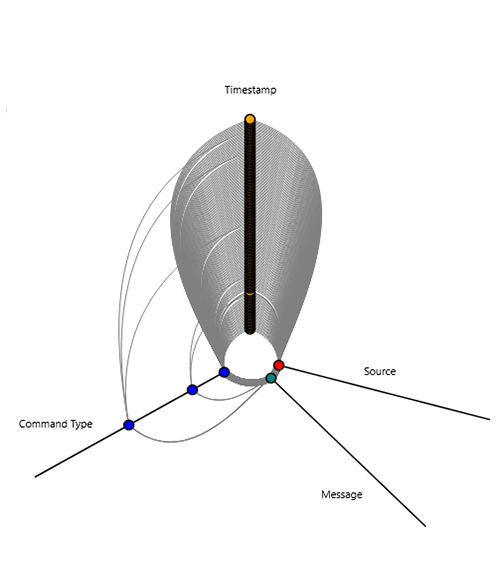
\includegraphics[width=2.5in]{images/regHive.png} 
   \caption{Hive plot displaying a random sample of 150 points from G-star logs. Data sampled is from February 6, 2017 -- May 25, 2017.}
   \label{fig:regHive}
\end{figure}
%% When citing figures in text IEEE wants them to be referenced as 'Fig. x' rather than Figure x
We gathered a simple random sample of 150 requests collected by the G-star logs between February 06, 2017 and May 25, 2017.  
This data was then rendered into a Hive plot~\cite{Hive-Plot} to interpret the attack. 
Hive plots are a perceptually uniform, scalable visualization for network analytics.  
We used a four-axis graph to reflect the relationships among timestamp, data source, command type, and response message (Fig.~\ref{fig:regHive}). 
The timestamp axis is the most heavily populated, containing distinct plotted points for each second during which a log entry was created. 
The source and message axes are closely related because there is only one plotted point on each axis. 
Source is the source of the response message returned by G-Star, and message is the response itself. 
In the context of the log file we analyzed, the source is always ``back-end'' (meaning the web server in this case) and message is always ``Unknown command:''. 
Lastly, the plotted points on the command type axis delineate unique HTTP request methods such as GET, POST, HEAD, PUT, DELETE, etc.

Fig.~\ref{fig:regHive} displays all 150 requests, while Fig.~\ref{fig:uniqHive} highlights the outlying requests that did not use the command type GET.  
Rather, these requests used the command types POST and HEAD. 
The POST requests are shown as the plotted point second closest to the center of the axis, while the HEAD requests are the farthest plotted point from the center of the axis. 
Fig.~\ref{fig:uniqHive} represents requests that used methods not commonly employed by web browsers or web crawlers, two of the most frequent sources of unwanted requests found in data gathered by Pasithea. 
This suggests these requests were deliberate and potentially malicious in nature.

\begin{figure}[t]
   \centering
   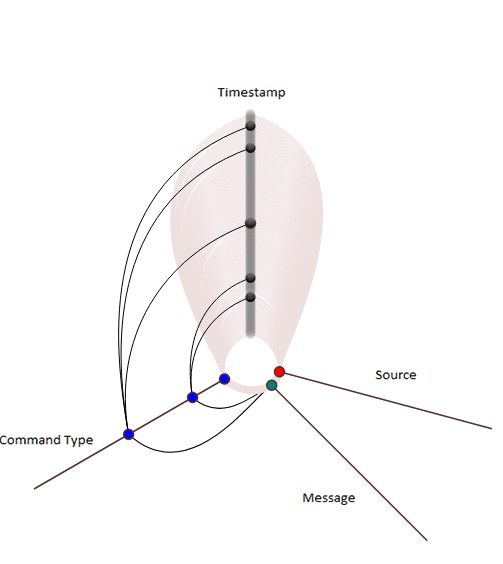
\includegraphics[width=2.5in]{images/uniqHive.png} 
   \caption{Hive plot where the prominent nodes denote ``injections'' into G-star that differ from normal traffic. Data sampled is from February 6, 2017 -- May 25, 2017}
   \label{fig:uniqHive}
\end{figure}

Cross-site scripting attacks aim to inject malicious scripts are injected into an otherwise benign or trusted website~\cite{XSS-def}. 
Further investigation of the specific commands being attempted as an XSS attack revealed the following:

\noindent \texttt{GET cgi\\
POST command.php\\
GET ;rm\$IFS-f\$IFS’'\\
GET ;wget\$IFS-O\$IFS’'\\
GET ;chmod\$IFS'’777’'\$IFS’'\\
GET ;sh\$IFS-c\$IFS‘'}

\noindent Fig. \ref{fig:XSS} displays a selected sample of entries collected by the G-star logs between March 11, 2017 and March 16, 2017. 
The highlighted requests have a span of 25 seconds where the XSS commands were attempted.
This shows both the short amount of time it took to run this malware insertion and the use of GET and POST request methods for one attack.
%% How do we get this to appear in the right column like earlier?
\begin{figure}[t]
   \centering
   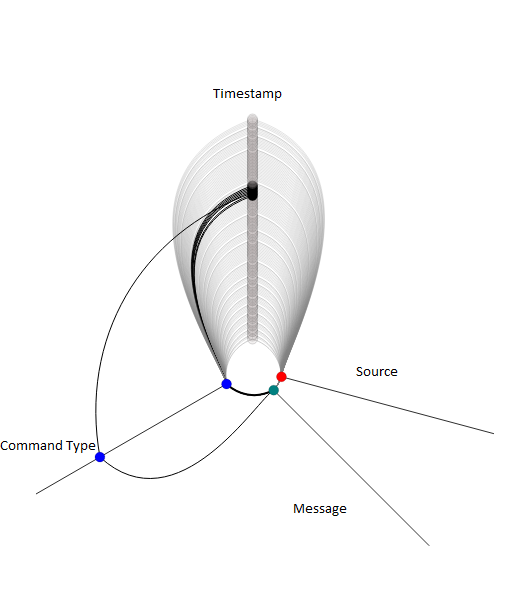
\includegraphics[width=2.5in]{images/XSS.png}  
   \caption{Hive plot where the prominent nodes display the XSS attempt on G-star. Data sampled is from March 11, 2017 -- March 16, 2017}
   \label{fig:XSS}
\end{figure}

We determined that a very similar attack sequence was also recently documented by a Finnish cyber-security company F-Secure~\cite{F-Secure}. 
The commands attempted with the XSS attack are intended to upload a PHP: Hypertext Preprocessor (PHP) file, then send a series of commands that, if executed, would remove a file using the \$IFS variable found in the PHP. 
Afterwards, it would attempt to download a file with the same variable name and change the permissions on said file so that it can be executed by any user.  
Then the attacker would execute the file. 
Researchers from F-Secure  attribute this attack profile to a Peer to Peer (P2P) botnet named TheMoon~\cite{TheMoon}. 
This example illustrates how we can use data collected from attack attempts to isolate and attribute the attack, provided that we can determine what types of attacks are taking place.

Pasithea was subsequently deployed and is currently active on our AWS EC2 instance in Ashburn, Virginia. 
Our log files indicate cursory web crawls from Baidu, a Chinese search engine, and some attempts at exploiting a known vulnerability in Apache Tomcat web servers using ``GET /manager/html''~\cite{Tomcat-Exploit}. 
We continue to monitor this instance, and additional results will be reported in a future paper.

%!TEX root=main.tex

\section{Construction Principles} \label{construction}

We developed Pasithea using Java, a common server-side programming language, and NanoHTTPD \cite{Nanohttpd}, a lightweight HTTP library written in Java that receives HTTP requests and returns responses.
Implementing this kind of functionality enables Pasithea to simulate a real application server in a lightweight and independent manner. 
It accepts any kind of request, regardless of the HTTP method, URI requested, or request body. 
Pasithea then logs the current time, the HTTP method, the path the client attempted to access (e.g. /index.html), the client's IP address, and the user agent data. 
Clients always receive a
 
% \texttt{<h1>404 Not Found</h1>}
% That's not working. Too bad.

\begin{center}  %% maybe \texttt ?
\texttt{$<$h1$>$404 Not Found$<$/h1$>$ }
\end{center}

\noindent
response, regardless of which resource they attempt to access.

In order to ensure attackers do not fingerprint Pasithea as a honeypot, we modeled our API honeypot after G-star Studio's ``real'' API.\footnote{
Please refer to the {\em ACM Inroads} article on G-star Studio~\cite{inroads-Labouseur16} for technical details about developing a Java-based REST API.
} 
But Pasithea always returns a 404 error, while G-star Studio, when prompted with a valid request, will return JSON-formatted data. 
The consistent 404 response is what makes Pasithea an unidentifiable, low-interaction honeypot. 
It is indistinguishable from a normal HTTP server whose valid URIs attackers do not know. 
%% In the future, we aim to extend Pasithea’s REST interface to extract more data from attackers while maintaining its cover as an unidentifiable API honeypot.

We are hosting our honeypot on an Amazon Web Services Elastic Compute Cloud (AWS EC2) instance using its ``free micro'' tier. 
We chose AWS both because of its appealing free tier model and because we were familiar with the security policies and standards that Amazon sets in place. 
We modified those default security policies within our AWS instance to enable access to the port hosting our API honeypot. 
Pasithea is currently indexed on Shodan~\cite{unsavoryChar}, a web search engine that indexes internetconnected devices.
Shodan is known for being frequented by the hacker community, making it likely that we will be able to collect additional attack data.

%!TEX root=main.tex

\section{Performance Tests} \label{performance}

Performance testing is a critical part of development, so it is important to demonstrate Pasithea's performance under different loads and its ability to log many -- potentially thousands -- of incoming requests in a short amount of time. 
In other words, it must respond fast enough to keep malicious users interested while also being stable enough to receive high volumes of incoming requests. 
To test this, we ran a series of benchmarks using the Apache Bench (ab) tool~\cite{ab}. 
This tool allows us to designate a number of completed requests to be sent to our API honeypot while varying the number of simulated concurrent users. 
The results from these tests are displayed in Fig.~\ref{fig:R/s} and Fig.~\ref{fig:T/R}. 

\begin{figure}[b]
   \centering
   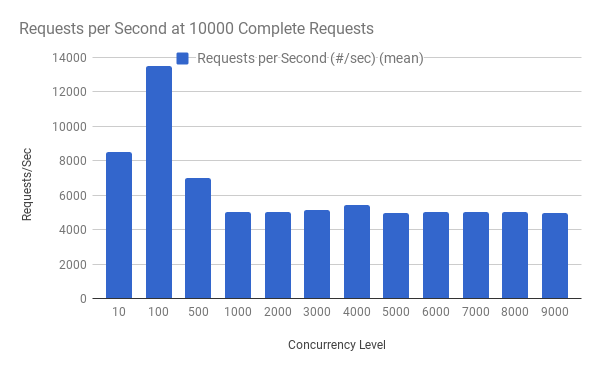
\includegraphics[width=2.5in]{images/RequestsperSecond.png} 
   \caption{Requests processed per second at varying concurrency levels}
   \label{fig:R/s}
\end{figure}

We researched a baseline response time for a RESTful API to give this data appropriate context. 
In doing so, we discovered two separate internal tests from software development and web monitoring companies, 3PillarGlobal~\cite{3Pillar} and Site24x7~\cite{site24x7}. 
Paired with some research on the human perception of performance~\cite{performance}, we concluded that a 300-ms response time is expected under normal traffic conditions in order for the API honeypot to appear realistic. 
Data collected on Pasithea indicates that we fall well within this range given a concurrency level of 500 simultaneous users. 
In addition, we continued tests at much higher concurrency levels to assess how well Pasithea would perform under extreme stress, like the attempts we saw on the G-star API. 
Pasithea can, with time, handle a concurrency level of over 9000 simultaneous requests while still logging more than 90\% of the requests received.

\begin{figure}[t]
   \centering
   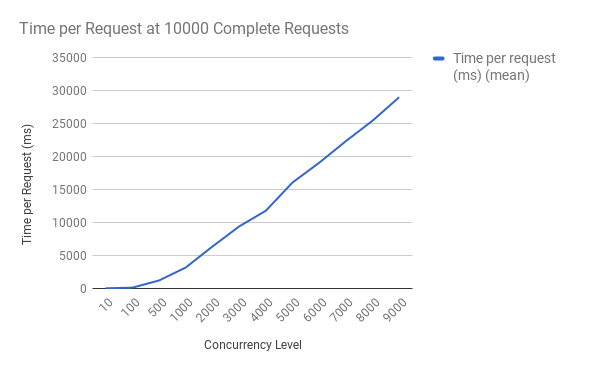
\includegraphics[width=2.5in]{images/TimeperRequest.png} 
   \caption{Mean time to complete a single request at varying concurrency levels}
   \label{fig:T/R}
\end{figure}

Since our implementation of request/response for Pasithea was deliberately kept very simple (only responding with 404 errors), we have thus far been unsuccessful in driving Pasithea hard enough during performance testing to reach a point where it is unable to handle a significant amount of requests.  
Pasithea hits a $R/s$ plateau at a concurrency level of 1000 (see Fig.~\ref{fig:R/s}), but continues to perform well at 9000.
With enough storage space, we believe that Pasithea could withstand a substantial attack, such as the one seen on G-star, and be able to log information about the attack for analysis.

%!TEX root=main.tex

\section{Conclusions and Future Work} \label{conclusions}

The API security landscape is more like a ``Wild West'' of conflicting standards than a safe, civilized, city of consistency.
This has led to an influx of attacks directed at APIs on many  fronts. 
Based on the attacks targeting G-star, the Dynamic Graph Database and our research into related attacks, we have constructed an API honeypot, Pasithea, with Java and NanoHTTPD to help combat and detail future attacks on the API landscape. 
Using hive plots and other tools, we have analyzed a real-world attack on G-star, demonstrating how DDoS and XSS attacks can be uncovered and attributed so that a proportionate defense may be deployed.  
Our performance data suggests that Pasithea should be able to keep a malicious user interested with fast response times while also maintaining composure and stability under high traffic loads. 
This allows us to develop accurate API attack profiles which will help shape the future of API security.

Our nest steps include . . .

% use section* for acknowledgement
\section*{Acknowledgments} \label{Acknowledgements}
The authors would like to thank Dayna Eidle and Thomas Famularo for their contributions in analyzing the data gathered from the G-star Graph Database, Mary Ann Hoffmann and Jonathan Heiles for reviewing this paper and contributing their thoughts from an outside perspective, and Thomas Magnusson for his help constructing Pasithea as well as reviewing and suggesting edits to the many drafts of this paper.

% can use a bibliography generated by BibTeX as a .bbl file
% BibTeX documentation can be easily obtained at:
% http://www.ctan.org/tex-archive/biblio/bibtex/contrib/doc/
% The IEEEtran BibTeX style support page is at:
% http://www.michaelshell.org/tex/ieeetran/bibtex/
%\bibliographystyle{IEEEtran}
% argument is your BibTeX string definitions and bibliography database(s)
%\bibliography{IEEEabrv,../bib/paper}
\bibliographystyle{ieeetran}
\bibliography{main}


% biography section
% 
% If you have an EPS/PDF photo (graphicx package needed) extra braces are
% needed around the contents of the optional argument to biography to prevent
% the LaTeX parser from getting confused when it sees the complicated
% \includegraphics command within an optional argument. (You could create
% your own custom macro containing the \includegraphics command to make things
% simpler here.)
%\begin{biography}[{\includegraphics[width=1in,height=1.25in,clip,keepaspectratio]{mshell}}]{Michael Shell}
% or if you just want to reserve a space for a photo:


%\begin{IEEEbiography}[{\includegraphics[width=1in,height=1.25in,clip,keepaspectratio]{picture}}]{John %Doe}
%\blindtext
%\end{IEEEbiography}


% You can push biographies down or up by placing
% a \vfill before or after them. The appropriate
% use of \vfill depends on what kind of text is
% on the last page and whether or not the columns
% are being equalized.


%\vfill


% Can be used to pull up biographies so that the bottom of the last one
% is flush with the other column.
%\enlargethispage{-5in}
% that's all folks
\end{document}

